\documentclass[a4paper, 14pt]{extarticle}
\usepackage{enumitem}
\usepackage{fefutitle}
\usepackage{listings}
\usepackage{xcolor}
\usepackage{amsmath}
\usepackage{graphicx}
\usepackage[justification=centering]{caption}
\usepackage{float}

\lstdefinestyle{mystyle}{
	basicstyle={\small\ttfamily},
	keywordstyle=\color{orange},
	stringstyle=\color{green},
	basicstyle=\ttfamily\footnotesize,
	breakatwhitespace=false,         
	breaklines=true,                 
	captionpos=b,                    
	keepspaces=true,                 
	numbers=none,                    
	numbersep=5pt,                  
	showspaces=false,                
	showstringspaces=false,
	showtabs=false,                  
	tabsize=2,
	aboveskip=3mm,
	belowskip=3mm,
}
\lstset{style=mystyle}

\begin{document}
	\fefutitle{1}
	\pagebreak	

	\section{Определение цели}
		В данной лабораторной необходимо создать математическую модель для выбора автомобиля в г. Владивосток автомобиля и рассчитать для неё:
		\begin{enumerate}[leftmargin=3\parindent, itemsep=0mm]
			\item минимальную мощность для езды
			\item мощность, для разгона до \(100 \text{км}/\text{ч} \)
		\end{enumerate}

	\section{Информация для создания модели}
		Город Владивосток имеет сложный рельеф: он расположен на холмах. Поэтому в модели необходимо рассматривать движение автомобиля по наклонной дороге.
		
		\(\alpha \) - угол наклона, в среднем составляет \( 15 ^\circ \)
		
		Рассмотрим два типа автомобиля: легковой и внедорожник.
		
		\( m \) - масса автомобиля. Зависит от типа кузова автомобиля:
		\begin{enumerate}[leftmargin=3\parindent, itemsep=0mm]
			\item Легковой автомобиль - 1250кг
			\item Внедорожник - 2250кг
		\end{enumerate}

		\( \upsilon \) - скорость автомобиля, варьируется от \(20 \text{км}/\text{ч} \) до \(60 \text{км}/\text{ч} \) 
		
		\( P \) - мощность автомобиля

	\section{Создание математической модели}
		\subsection{Движение под углом}
			Рассмотрим движение автомобиля по наклонной дороге:
			\( S \) - расстояние, пройденное автомобилем
			\[ S = \upsilon \Delta t \tag{3.1.1} \label{eq:special} \]
			, где \( \Delta t \) - время, за которое автомобиль проезжает расстояние S,
			\( \upsilon \) - скорость движения
	
			Высота, на которую поднимается автомобиль, вычисляется по формуле
			\[ h = S \cdot \sin{\alpha} \tag{3.1.2} \label{eq:special}\]
			Подставим \( (3.1.1) \) в (3.1.2):
			\[ h = \upsilon \Delta t \cdot sin{\alpha}  \tag{3.1.3} \label{eq:special} \]
			Мощность найдём из закона сохранения энергии, не учитывая силу трения
			\[ P \Delta t = mgh  \tag{3.1.4} \label{eq:special}\]
			, где \( g \) - скорость свободного падения(\( g \approx 9.8 \))
			
			Выразим \( \Delta t\) из (3.1.3)
			\[ \Delta t = \dfrac{h}{\upsilon \sin{\alpha}} \tag{3.1.5} \label{eq:special} \]
			и подставим в (3.1.4) и получим
			\[ P = mg \upsilon \sin{\alpha} \tag{3.1.6} \label{eq:special} \]
		\subsection{Движение по прямой}
			Для вычисления мощности при движении по прямой воспользуемся
			законом сохранения энергии
			\[ P \Delta t = \dfrac{m\upsilon^2}{2} \tag{3.2.1} \label{eq:special} \]
			Выразим P
			\[ P = \dfrac{m\upsilon^2}{2\Delta t} \tag{3.2.2} \label{eq:special} \]

	\section{Анализ модели}
		Программы были написаны на языке Java с использованием Python-библиотеки matplotlib для построение графиков.
		\subsection{Движение под углом}
			\begin{enumerate}
				\item Зависимость мощности от скорости движения под углом \( 15^\circ \)
				
				Код программы:
				\begin{lstlisting}[language=Java]
public class Main {
	private static final Double g = 9.8;
	
	private final static Double horsePowerDelimeter = 735.499;
	
	private static Double toHorsePower(Double power) {
		return power/horsePowerDelimeter;
	}
	
	private static Double toMeterForSecond(Double v) {
		return v * 1000/3600;
	}
	
	public static Double powerInHorsePowersAlpha(Double m, Double v, Double alpha) {
		return toHorsePower(m*g*toMeterForSecond(v)*Math.sin(Math.toRadians(alpha)));
	}
	
	public static void main(String[] args) throws PythonExecutionException, IOException {
		ArrayList<Double> vs = new ArrayList<>();
		ArrayList<Double> ps1 = new ArrayList<>();
		ArrayList<Double> ps2 = new ArrayList<>();
		for(double v = 20.; v <= 60; ++v) {
			vs.add(v);
			ps1.add(powerInHorsePowersAlpha(1250., v, 15.));
			ps2.add(powerInHorsePowersAlpha(2250., v, 15.));
		}
		Plot plt = Plot.create();
		plt.plot().add(vs, ps1).linewidth(2.);
		plt.plot().add(vs, ps2).linewidth(2.);
		plt.xlabel("V");
		plt.ylabel("P");
		plt.legend();
		plt.show();
	}
}
				\end{lstlisting}
				\begin{figure}[H]
					\centering
					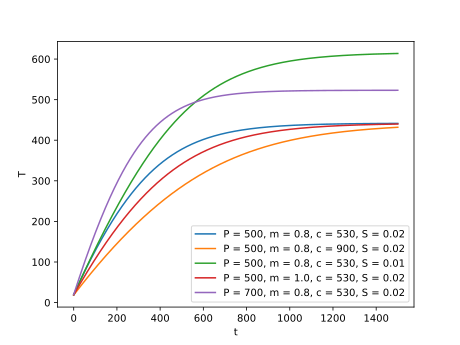
\includegraphics[width = \linewidth]{fig1.pdf}
					\caption[.] {График зависимости P от \( \upsilon \)}
				\end{figure}
				При \( \alpha = 15^\circ \) для того, чтобы двигаться 
				cо скоростью \( \upsilon = 20 \text{км}/\text{ч} \) легковой машине необходима P = 24 л.с.,
				внедорожнику P = 44 л.с. 
				\pagebreak
				\item Зависимость мощности от массы при скорости \( \upsilon = 20 \text{км}/\text{ч} \)
				
					Т.к. масса легкового автомобиля в среднем варьируется от 1000кг до 1500кг, а внедорожника до 2500кг, то построим график зависимости мощности от массы автомобиля.
					Код программы:
					\begin{lstlisting}[language=Java]
public class Main {
	private static final Double g = 9.8;
	
	private final static Double horsePowerDelimeter = 735.499;
	
	private static Double toHorsePower(Double power) {
		return power/horsePowerDelimeter;
	}
	
	private static Double toMeterForSecond(Double v) {
		return v * 1000/3600;
	}
	
	public static Double powerInHorsePowersAlpha(Double m, Double v, Double alpha) {
		return toHorsePower(m*g*toMeterForSecond(v)*Math.sin(Math.toRadians(alpha)));
	}
	
	public static void main(String[] args) throws PythonExecutionException, IOException {
		ArrayList<Double> vs = new ArrayList<>();
		ArrayList<Double> ps1 = new ArrayList<>();
		
		for(double m = 1000; m <= 2500; ++m) {
			vs.add(m);
			ps1.add(powerInHorsePowersAlpha(m, 40., 15.));
		}
		Plot plt3 = Plot.create();
		plt3.plot().add(vs, ps1).linewidth(2.);
		plt3.xlabel("m");
		plt3.ylabel("P");
		plt3.legend();
		plt3.show();
	}
}
					\end{lstlisting}
					\begin{figure}[H]
						\centering
						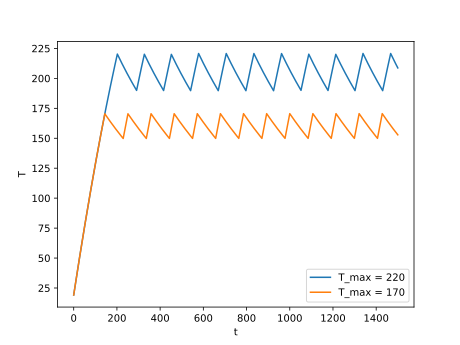
\includegraphics[width = \linewidth]{fig2.pdf}
						\caption[.] {График зависимости P от m при \( \upsilon = 40 \text{км}/\text{ч} \)}
					\end{figure}
			\end{enumerate}
		\pagebreak
		\subsection{Движение по прямой}
			Посмотрим график разгона легковой машины с m = 1250кг до 100 км/ч 
			
			Код программы:
			\begin{lstlisting}[language=Java]
public class Main {
	private static final Double g = 9.8;
	
	private final static Double horsePowerDelimeter = 735.499;
	
	private static Double toHorsePower(Double power) {
		return power/horsePowerDelimeter;
	}
	
	private static Double toMeterForSecond(Double v) {
		return v * 1000/3600;
	}
	
	public static Double powerInHorsePowersStraight(Double m, Double v, Double t) {
		return toHorsePower(m*Math.pow(toMeterForSecond(v), 2) / (2*t));
	}
	
	public static void main(String[] args) throws PythonExecutionException, IOException {
		ArrayList<Double> vs = new ArrayList<>();
		ArrayList<Double> ps1 = new ArrayList<>();
		for(double t = 3; t <= 5; t += 0.1) {
			vs.add(t);
			ps1.add(powerInHorsePowersStraight(1250., 100., t));
		}
		Plot plt2 = Plot.create();
		plt2.plot().add(vs, ps1).linewidth(2.);
		plt2.xlabel("t");
		plt2.ylabel("P");
		plt2.legend();
		plt2.show()
	}
			\end{lstlisting}
			\begin{figure}[H]
				\centering
				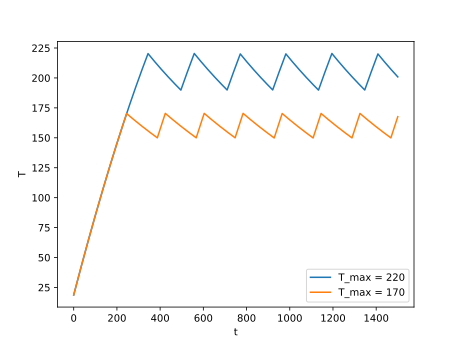
\includegraphics[width = \linewidth]{fig3.pdf}
				\caption[.] {График зависимости P от t при разгоне до100 км/ч}
			\end{figure}
			Для разгона автомобиля массой 1250кг за 5 секунд до 100км/ч в 
			построенной математической модели требуется мощность P = 131л.с.
			В реальности, например Tesla Model 3 с такими же параметрами, имеет P = 280 л.с.
			Такая разница получается из-за того, что в модели не учитываются такие важные параметры
			как: сила трения и сопротивление воздуха.
			\begin{figure}[H]
				\centering
				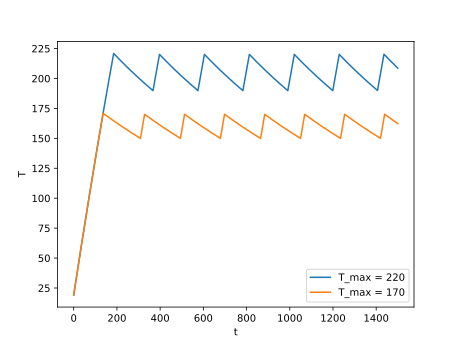
\includegraphics[width = \linewidth]{fig4.png}
				\caption[.] {Tesla Model 3}
			\end{figure}
		\section{Вывод}
			В данной лабораторной работе была составлена простая математическая модель автомобиля,
			а также с помощью модели установили зависимость мощности автомобиля от скорости и массы
			при движении под углом и зависимость мощности от времени, при разгоне до 100 км/ч.
\end{document}	